\documentclass[12pt]{article}
\usepackage{amssymb,amsmath}% http://ctan.org/pkg/{amssymb,amsmath}
\usepackage{braket}% http://ctan.org/pkg/braket
\usepackage[margin=0.1in]{geometry}
\usepackage{graphicx}
\usepackage{subcaption}
\usepackage{amsmath}
\usepackage{relsize}
\begin{document}





\[\text{\bf{Customer C Spend on Order X}} = c*r*t + \epsilon \]
\[c = \text{Customer's mean order amount in dollars where } c \sim \mathcal{N}(\$100,\$25).\]
\[r = \text{Scalar corresponding to mean retailer order amount where } r \sim \mathcal{N}(1.0,0.05).\]
\[t = \text{Whether or not the customer recieved the experimental treatment } t \in [1,1.01].\]
\[\epsilon = \text{Random noise where } \epsilon \sim \mathcal{N}(\$10,\$1).\]
\[\text{The number of orders placed by Customer C }  \sim exp(\lambda = 1).\]


\newpage
\begin{table}[]
\begin{tabular}{c|ccccccccc}
                                                                              & \textbf{\begin{tabular}[c]{@{}c@{}}Method \\ I\end{tabular}} & \textbf{\begin{tabular}[c]{@{}c@{}}Method \\ II\end{tabular}} & \textbf{\begin{tabular}[c]{@{}c@{}}Method\\ III\end{tabular}} & \textbf{\begin{tabular}[c]{@{}c@{}}Method \\ IV\end{tabular}} & \textbf{\begin{tabular}[c]{@{}c@{}}Method \\ V\end{tabular}} & \textbf{\begin{tabular}[c]{@{}c@{}}Method \\ VI\end{tabular}} & \textbf{\begin{tabular}[c]{@{}c@{}}Method \\ VII\end{tabular}} & \textbf{\begin{tabular}[c]{@{}c@{}}Method \\ VIII\end{tabular}} & \textbf{\begin{tabular}[c]{@{}c@{}}Method \\ IX\end{tabular}} \\ \hline
\textbf{Simulations Required}                                                 & T                                                            & F                                                             & T                                                             & T                                                             & T                                                            & s                                                             & s                                                              & s                                                               & s                                                             \\ \hline
\textbf{Mean Time Required}                                                   & T                                                            & F                                                             & F                                                             & T                                                             & T                                                            & s                                                             & s                                                              & s                                                               & s                                                             \\ \hline
\textbf{\begin{tabular}[c]{@{}c@{}}Mean Error \\ (Est. Power)\end{tabular}}   & F                                                            & T                                                             & T                                                             & T                                                             & T                                                            & s                                                             & s                                                              & s                                                               & s                                                             \\ \hline
\textbf{\begin{tabular}[c]{@{}c@{}}Std. of Error\\ (Est. Power)\end{tabular}} & F                                                            & T                                                             & F                                                             & F                                                             & F                                                            & s                                                             & s                                                              & s                                                               & s                                                            
\caption[short]{Intel Xeon(R) CPU E5-2670}
\end{tabular}
\end{table}

\newpage

\noindent
\begin{figure}[b]
\centering
\begin{subfigure}{.32\textwidth}
    \centering
    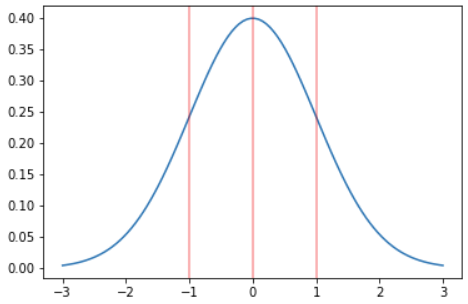
\includegraphics[width=0.75\textwidth]{sd_3.png}
    \caption[short]{$\mu$ +/- [1]$\sigma$ \\with 500 iterations.}
    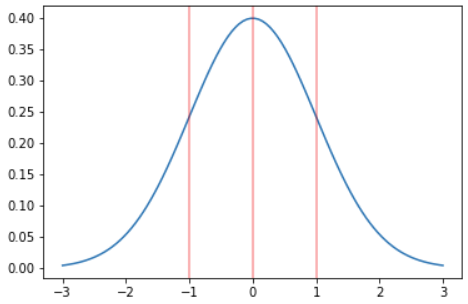
\includegraphics[width=0.75\textwidth]{sd_3.png}
    \caption[short]{$\mu$ +/- [1,2]$\sigma$ \\with 500 iterations.}
    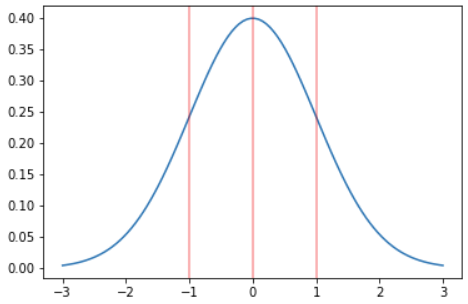
\includegraphics[width=0.75\textwidth]{sd_3.png}
    \caption[short]{$\mu$ +/- [1,2,3]$\sigma$ \\with 500 iterations.}
\end{subfigure}
\begin{subfigure}{.32\textwidth}
    \centering
    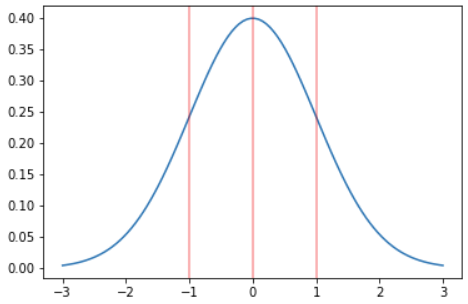
\includegraphics[width=0.75\textwidth]{sd_3.png}
    \caption[short]{$\mu$ +/- [1]$\sigma$ \\with 1,000 iterations.}
    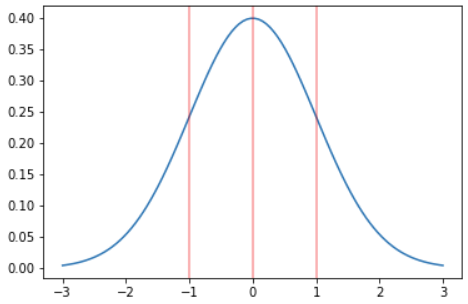
\includegraphics[width=0.75\textwidth]{sd_3.png}
    \caption[short]{$\mu$ +/- [1,2]$\sigma$ \\with 1,000 iterations.}
    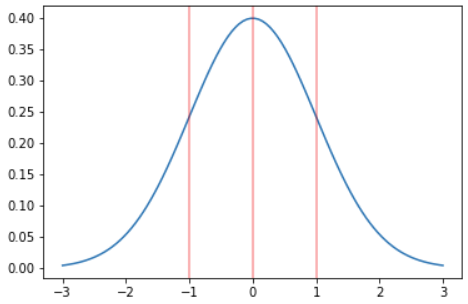
\includegraphics[width=0.75\textwidth]{sd_3.png}
    \caption[short]{$\mu$ +/- [1,2,3]$\sigma$ \\with 1,000 iterations.}
\end{subfigure}
\begin{subfigure}{.32\textwidth}
    \centering
    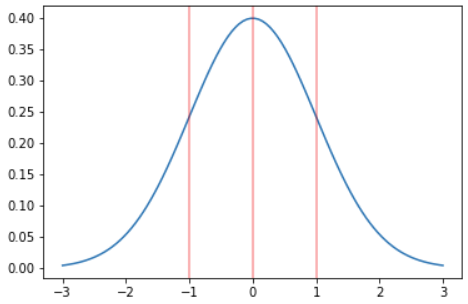
\includegraphics[width=0.75\textwidth]{sd_3.png}
    \caption[short]{$\mu$ +/- [1]$\sigma$ \\with 2,000 iterations.}
    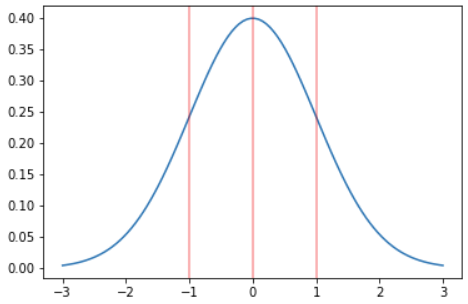
\includegraphics[width=0.75\textwidth]{sd_3.png}
    \caption[short]{$\mu$ +/- [1,2]$\sigma$ \\with 2,000 iterations.}
    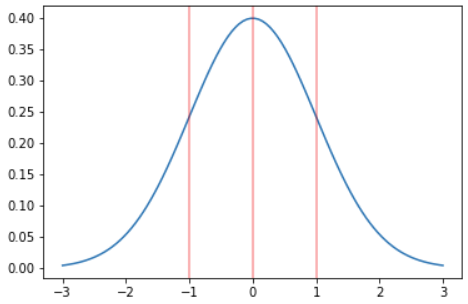
\includegraphics[width=0.75\textwidth]{sd_3.png}
    \caption[short]{$\mu$ +/- [1,2,3]$\sigma$ \\with 2,000 iterations.}
\end{subfigure}%
\caption[short]{Intel® Xeon(R) CPU E5-2670}
\end{figure}


\newpage
If we were implementing a difference of means t-test, then we could simply apply the formula below to get the appropriate sample size.
\[n = 2 \Bigg(\frac{Z_{1-(\alpha/2)}+Z_{1-\beta}}{ES}\Bigg)^2 \text{  where  } ES = \frac{|\mu_1-\mu_2|}{\sigma}\]

Here, $\alpha$ is the probability of a Type I error (false rejection of the NULL hypothesus, i.e. a false positive) and $\beta$ is the probability of a Type II error (i.e. a false negative). Observe how if we want to make our test more rigorous and reduce the false positive rate, the the left side of the numerator increase and the resulting recommended sample size - $n$, also increases. Similarly, if we want to reduce the probability for failing to detect the difference across groups, then we will need to increase the right-hand side of the numerator - also increasing the recommended sample size.

\newpage
\[ y = \beta_0 + \mathlarger{\mathlarger{\mathlarger{\mathlarger{\mathlarger{\mathlarger{\epsilon}}}}}} \]
\[ y = \beta_0 + X_1\beta_1 + \mathlarger{\mathlarger{\mathlarger{\epsilon}}}\]
\[ y = \beta_0 + X_1\beta_1 + X_2\beta_2 + \mathlarger{\mathlarger{\epsilon}}\]
\[ y = \beta_0 + X_1\beta_1 + X_2\beta_2 + X_3\beta_3 +\mathlarger{\epsilon}\]
\[ y = \beta_0 + ... + \beta_nX_n + \epsilon \text{\phantom{aa} where \phantom{aa}} \epsilon = \hat{y} - y\]

\newpage
\[Y = \text{Signal} + \text{Noise}_{\text{clustered}} + \text{Noise}_{\text{unclustered}} \]

%\[Y = \text{Signal} + \text{Explained Noise}_{\text{clustered}} + \text{Unexplained Noise}_{\text{clustered}} +  \n \text{Explained Noise}_{\text{unclustered}} +  \text{Unexplained Noise}_{\text{clustered}}\]

\begin{center}
\begin{multline}
Y = \text{Signal} + \text{Explained Noise}_{\text{clustered}} + \\
\phantom{a} =  \text{Unexplained Noise}_{\text{clustered}} 
\end{multline}
\end{center}


\end{document}